\documentclass[tikz,border=0pt]{standalone}
\usepackage{lmodern}
\definecolor{ink}{HTML}{12394B}
\definecolor{grid}{HTML}{284C5B}
\definecolor{area}{HTML}{427A7B}
\definecolor{stripe}{HTML}{76AAA0}
\definecolor{axis}{HTML}{ADC5CB}
\definecolor{chalk}{HTML}{F5F8EF}
\definecolor{gold}{HTML}{FFD07C}
\begin{document}
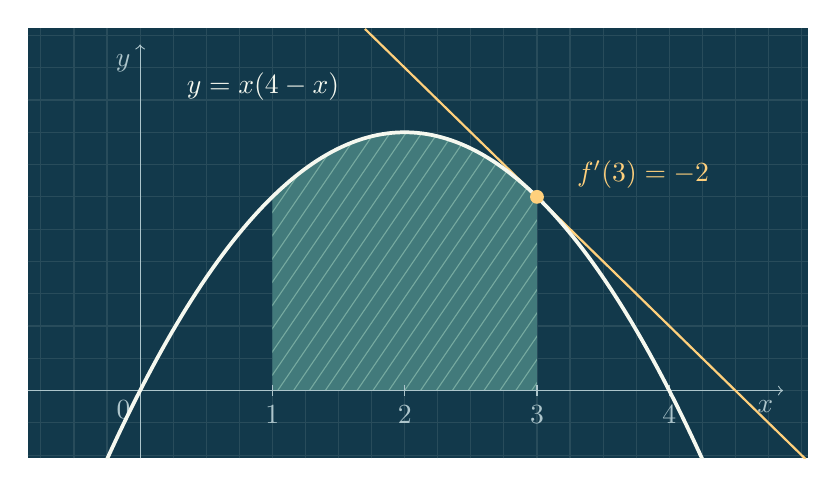
\begin{tikzpicture}[x=1.68cm,y=.82cm]
  \clip (-.85,-1.05) rectangle (5.05,5.62);
  \fill[ink] (-.85,-1.05) rectangle (5.05,5.62);
  \draw[grid,thin,xstep=.42cm,ystep=.41cm] (-.85,-1.05) grid (5.05,5.62);
  \begin{scope}
    \clip (1,0) -- plot[domain=1:3,samples=65] (\x,{\x*(4-\x)}) -- (3,0) -- cycle;
    \fill[area] (1,0) rectangle (3,4.1);
    \foreach \a in {-1,-.88,...,3}
      \draw[stripe,thin] (\a,0) -- (\a+1.4,4.2);
  \end{scope}
  \draw[axis,->] (-.85,0) -- (4.86,0) node[below left] {$x$};
  \draw[axis,->] (0,-1.05) -- (0,5.36) node[below left] {$y$};
  \foreach \a in {1,2,3,4}
    \draw[axis] (\a,.09) -- (\a,-.09) node[below] {$\a$};
  \node[axis,below left] at (0,0) {$0$};
  \draw[gold,thick] (1.70,5.60) -- (5.03,-1.06);
  \draw[chalk,line width=1.35pt] plot[domain=-.25:4.25,samples=120] (\x,{\x*(4-\x)});
  \fill[gold] (3,3) circle[radius=2.5pt];
  \node[chalk,anchor=south west] at (.28,4.34) {$y=x(4-x)$};
  \node[gold,anchor=west] at (3.23,3.35) {$f'(3)=-2$};
\end{tikzpicture}
\end{document}
